\begin{figure}[htp]
	\centering
	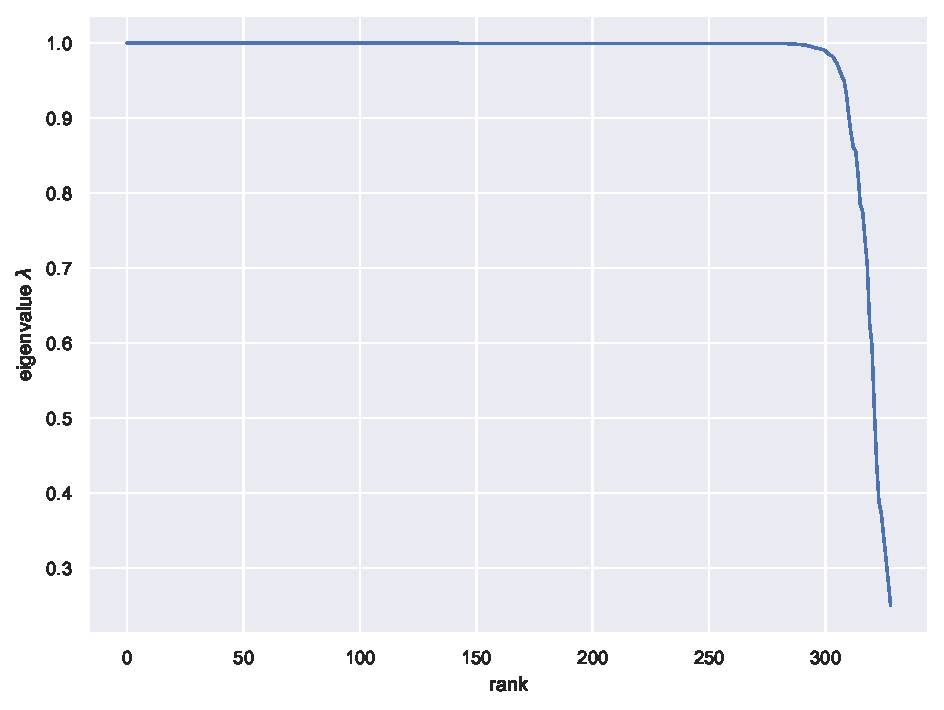
\includegraphics[width=\textwidth]{homer_slepian_eigenvalues_b1275.pdf}
	\caption[
		The Slepian eigenvalues of the Homer head region
	]{
		The eigenvalues of the Homer head region concentrated within the Shannon number \(N=329\).
		The majority of the eigenvalues are \(\almost{1}\) before decreasing rapidly towards zero around the Shannon number.
	}\label{fig:chapter4_slepian_eigenvalues}
\end{figure}
